\section{Time integration}
In the previous sections we described various methods of calculating forces applied to particles in the simulation.
Once these forces are found, the evolution of the system in time can be tracked by integrating Newton's 2nd law of motion,
\begin{equation}\label{eq:newtons-second}
    \ddot{\mathbf{x}}_i = \frac{\mathbf{F}_i}{m_i}.
\end{equation}

\subsection{Euler's method}
Possibly, the simplest numerical method that could be used is Euler's method described by the update rules
\begin{equation}\label{eq:eulers-method}
    \begin{aligned}
        \mathbf{v}_i^{(k+1)} & = \mathbf{v}_i^{(k)} + \textrm{DT} \frac{\mathbf{F}^{(k+1)}_i}{m_i}, \\
        \mathbf{x}_i^{(k+1)} & = \mathbf{x}_i^{(k)} + \textrm{DT} \mathbf{v}_i^{(k)}.
    \end{aligned}
\end{equation}
The method defined in \autoref{eq:eulers-method} is not suitable for physical simulations, however.
Its shortcomings are best illustrated by an example of an undamped pendulum of length $l$ in gravitational field of magnitude $g$.
Although it is a simple system, it illustrates the numerical challenges faced in gravitational simulations over long timescales, particularly the issue of energy preservation.

The motion of the pendulum is governed by the differential equation
\begin{equation*}
    \ddot{\theta} = -\frac{g}{l}\sin\theta,
\end{equation*}
and its kinetic and potential energy are given by $\textrm{KE} = (1/2)ml^2\dot{\theta}$ and $\textrm{PE} = -mgl\cos\theta$ respectively.
\begin{figure}[htp]
    \centering
    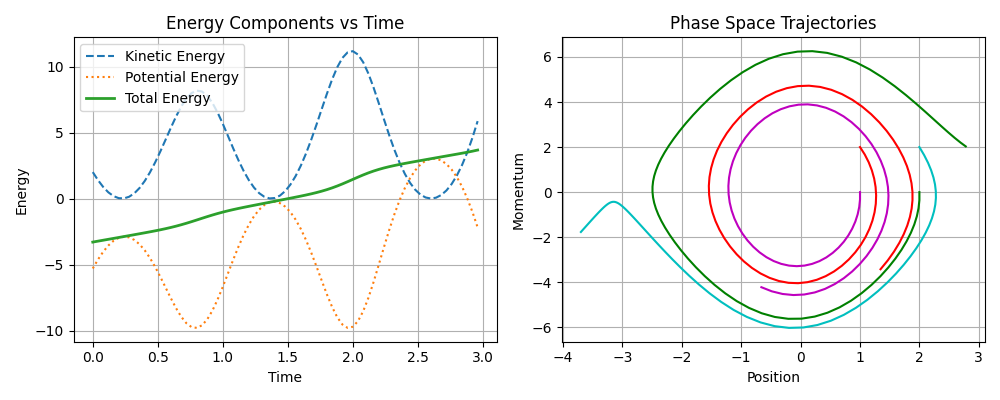
\includegraphics[scale=0.6]{img/integrators/euler-pendulum.png}
    \caption{Behavior of Euler's method: lack of conservation of energy and phase space trajectories spiraling out.}
    \label{fig:euler-integrator}
\end{figure}
As shown in \autoref{fig:euler-integrator}, Euler's method fails to conserve total energy $(\textrm{PE} + \textrm{KE})$ and produces trajectories in phase space that are not closed, contrary to expectations for periodic systems.
Additionally, the evolution of an area element in phase space violates Liouville's theorem, as described in \cite{taylor2005classical}, making the method unsuitable for long-term physical simulations (see \autoref{fig:area-euler-vs-leapfrog}).
\begin{figure}[htp]
    \centering
    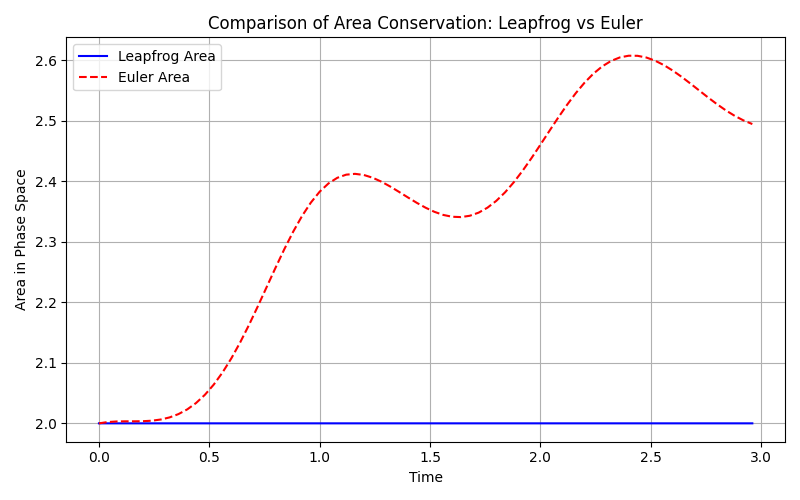
\includegraphics[scale=0.4]{img/integrators/area-leap-vs-euler.png}
    \caption{Area in phase space over time. Violation of Liouville's theorem by Euler's method.}
    \label{fig:area-euler-vs-leapfrog}
\end{figure}

\subsection{Leapfrog algorithm}
The leapfrog algorithm, given by the update rule \cite{young_leapfrog_2019}
\begin{equation}\label{eq:leapfrog}
    \begin{aligned}
        \mathbf{v}_{i}^{(1/2)} & = \mathbf{v}_i^{(0)} + \frac{1}{2}\textrm{DT} \frac{\mathbf{F}_i^{(0)}}{ m_i^{(0)}}, \\
        \mathbf{x}_i^{(k+1)}   & = \mathbf{x}_i^{(k)} + \textrm{DT} \mathbf{v}_i^{(k+1/2)},                           \\
        \mathbf{v}_i^{(k+3/2)} & = \mathbf{v}_i^{(k+1/2)} + \textrm{DT} \frac{ \mathbf{F}_i^{(k+1)}}{m_i}.
    \end{aligned}
\end{equation}
is the preferred way of integrating \autoref{eq:newtons-second}.
When applied to the same pendulum system, it conserves energy much more faithfully and preserves the area in phase space, consistent with Liouville's theorem (see \autoref{fig:leapfrog-integrator} and \autoref{fig:area-euler-vs-leapfrog}).
\begin{figure}[htp]
    \centering
    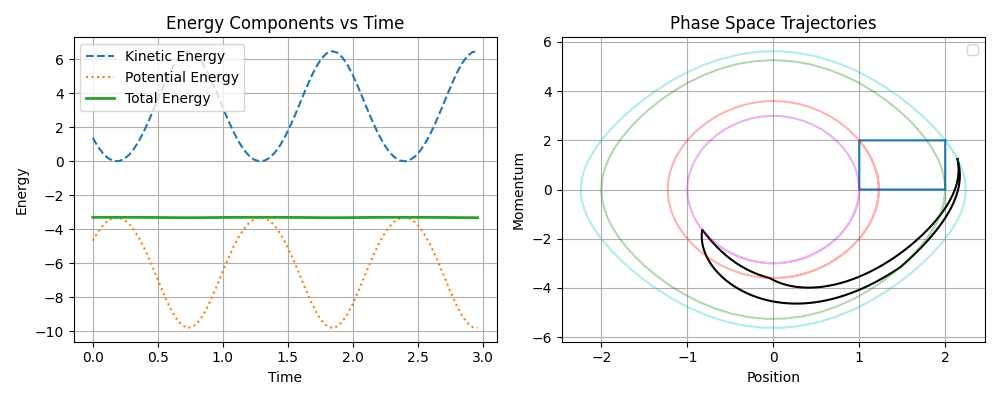
\includegraphics[scale=0.6]{img/integrators/leapfrog-pendulum.png}
    \caption{Behavior of the leapfrog algorithm: conservation of energy and phase space trajectories forming closed loops.
        Evolution of an area element in phase space is shown on the right-hand side: blue rectangle -- initial conditions for many copies of the system; black distorted quadrilateral -- their state by the end of the simulation.}
    \label{fig:leapfrog-integrator}
\end{figure}
Given its simplicity and excellent long-term energy behavior, we adopt the leapfrog algorithm to integrate Newton's equations in our program.